\subsubsection{Persistence Layer}

\begin{figure}[H]
    \centering
    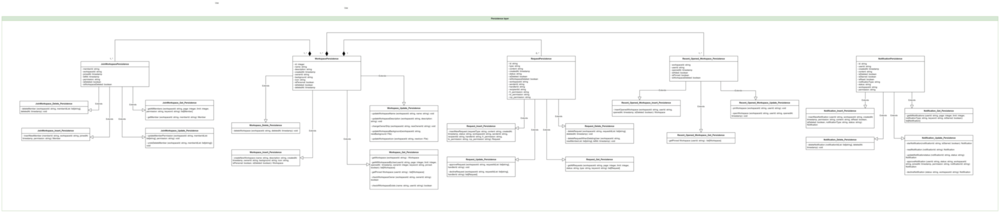
\includegraphics[ width = \linewidth]{Content/Phân tích và thiết kế hệ thống/documents/Sơ đồ lớp/images/Persistence layer/persistenceLayer.png}
    \vspace{0.5cm}
    \caption{Persistence Layer}
    \label{fig:Persistence Layer}
\end{figure}
Tầng Persistence sẽ nhận dữ liệu, yêu cầu từ tầng Business để thực hiện các thao tác tương tác với cơ sở dữ liệu, sau đó trả về kết quả cho tầng Business.

\begin{figure}[H]
    \centering
    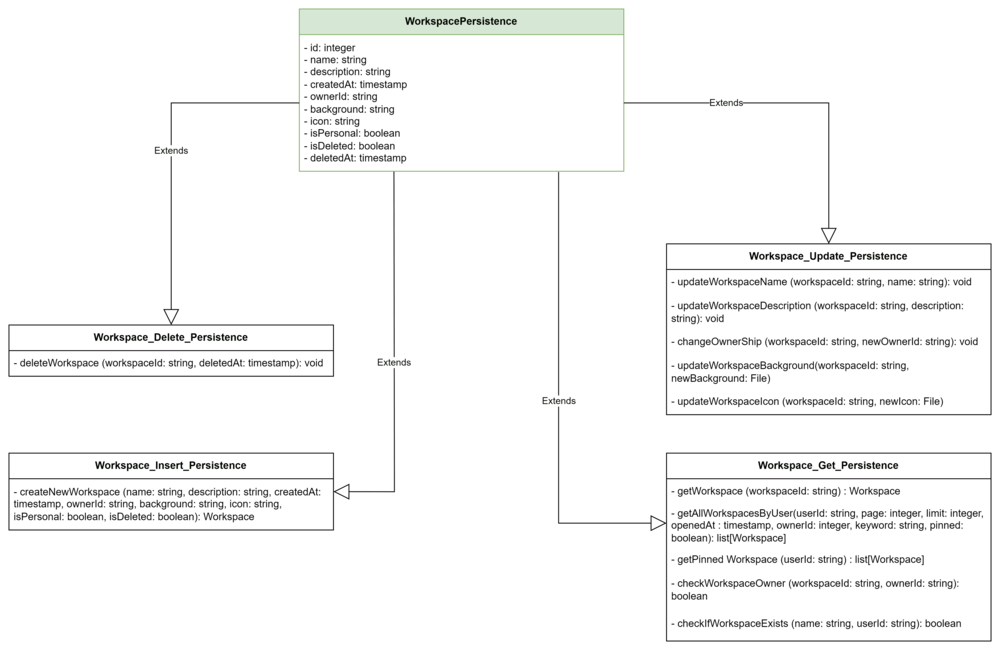
\includegraphics[ width = \linewidth]{Content/Phân tích và thiết kế hệ thống/documents/Sơ đồ lớp/images/Persistence layer/workspacePersistence.png}
    \vspace{0.5cm}
    \caption{Workspace Persistence}
    \label{fig:Workspace Persistence}
\end{figure}

\begin{figure}[H]
    \centering
    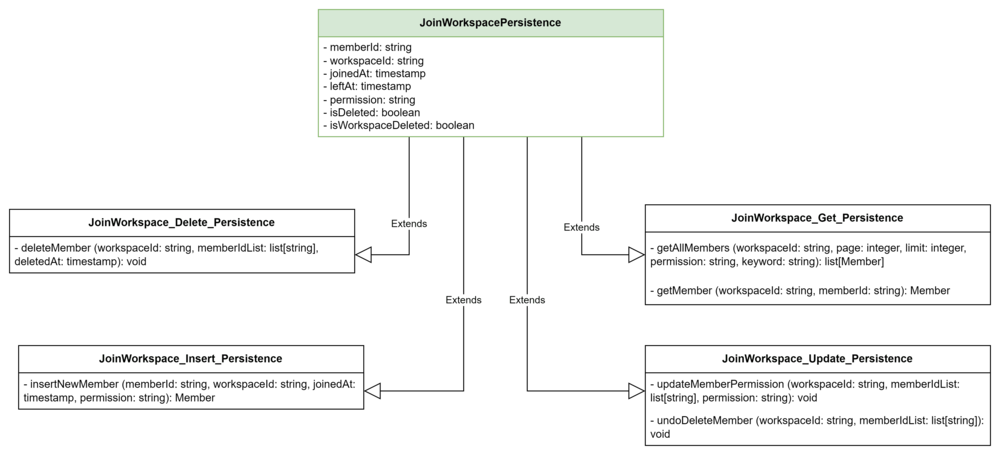
\includegraphics[ width = \linewidth]{Content/Phân tích và thiết kế hệ thống/documents/Sơ đồ lớp/images/Persistence layer/joinWorkspacePersistence.png}
    \vspace{0.5cm}
    \caption{Join Workspace Persistence}
    \label{fig:Join Workspace Persistence}
\end{figure}

\begin{figure}[H]
    \centering
    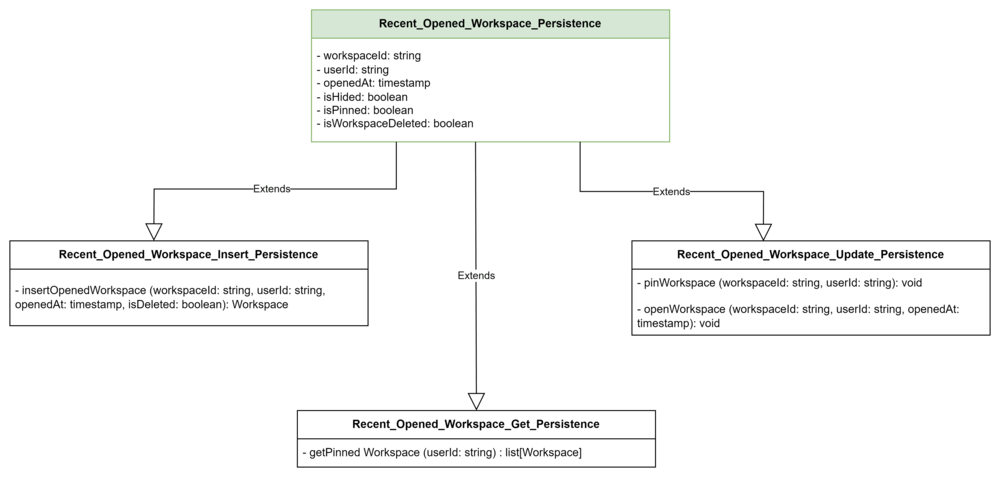
\includegraphics[ width = \linewidth]{Content/Phân tích và thiết kế hệ thống/documents/Sơ đồ lớp/images/Persistence layer/recentOpenedWorkspacePersistence.png}
    \vspace{0.5cm}
    \caption{Recent Opened Workspace Persistence}
    \label{fig:Recent Opened Workspace Persistence}
\end{figure}

\begin{figure}[H]
    \centering
    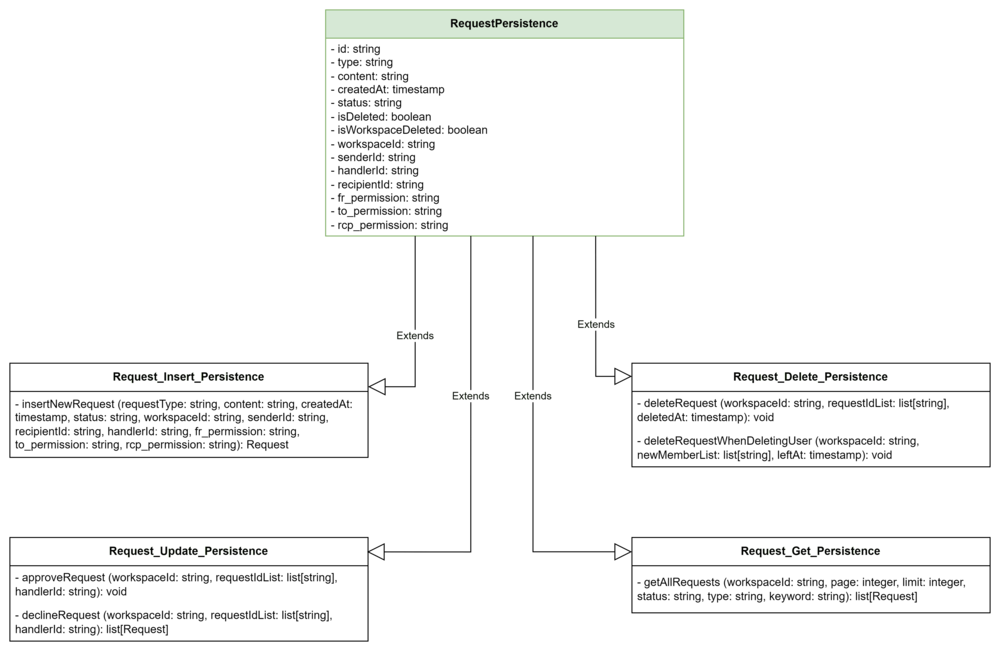
\includegraphics[ width = \linewidth]{Content/Phân tích và thiết kế hệ thống/documents/Sơ đồ lớp/images/Persistence layer/requestPersistence.png}
    \vspace{0.5cm}
    \caption{Request Persistence}
    \label{fig:Request Persistence}
\end{figure}

\begin{figure}[H]
    \centering
    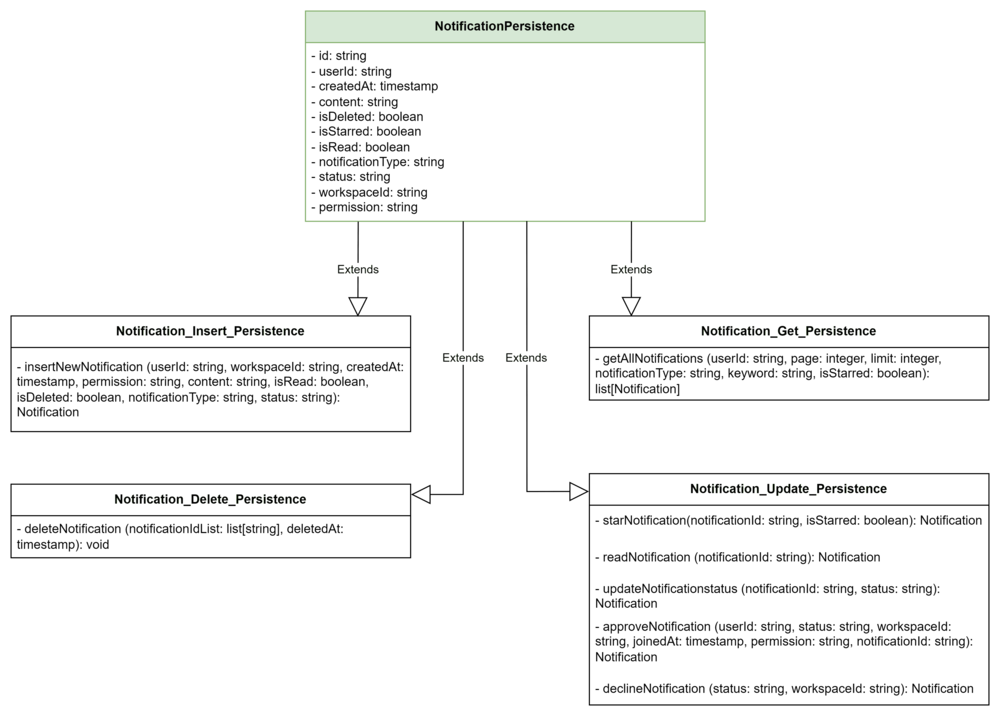
\includegraphics[ width = \linewidth]{Content/Phân tích và thiết kế hệ thống/documents/Sơ đồ lớp/images/Persistence layer/notificationPersistence.png}
    \vspace{0.5cm}
    \caption{Notification Persistence}
    \label{fig:Notification Persistence}
\end{figure}